\documentclass[DIN, pagenumber=false, fontsize=11pt, parskip=half]{scrartcl}

\usepackage{amsmath}
\usepackage{amsfonts}
\usepackage{amssymb}
\usepackage{enumitem}
\usepackage[utf8]{inputenc} 
\usepackage[ngerman]{babel} 
\usepackage[T1]{fontenc} 
\usepackage{pgfplots}
\usepackage{xcolor}
\usepackage{listings}
\usepackage{float}
\usepackage{graphicx}
\usepackage{booktabs}
\usepackage{tkz-euclide}
\usepackage{svg}
\usepackage{trfsigns}
\usepackage{mathtools}

\DeclarePairedDelimiter\abs{\lvert}{\rvert}%
\DeclarePairedDelimiter\norm{\lVert}{\rVert}%

\definecolor{mygreen}{RGB}{28,172,0} % color values Red, Green, Blue
\definecolor{mylilas}{RGB}{170,55,241}

\tikzstyle{neuron}=[circle,fill=black!25,minimum size=30pt,inner sep=0pt]

\lstset{language=Matlab,%
    %basicstyle=\color{red},
    breaklines=true,%
    morekeywords={matlab2tikz},
    keywordstyle=\color{blue},%
    morekeywords=[2]{1}, keywordstyle=[2]{\color{black}},
    identifierstyle=\color{black},%
    stringstyle=\color{mylilas},
    commentstyle=\color{mygreen},%
    showstringspaces=false,%without this there will be a symbol in the places where there is a space
    numbers=left,%
    numberstyle={\tiny \color{black}},% size of the numbers
    numbersep=9pt, % this defines how far the numbers are from the text
    emph=[1]{for,end,break},emphstyle=[1]\color{red}, %some words to emphasise
    %emph=[2]{word1,word2}, emphstyle=[2]{style},    
}

\title{Einführung in die Neuroinformatik}
\author{Tim Luchterhand, Paul Nykiel (Gruppe P)}

\begin{document}
    \maketitle
    \section{Transferfunktionen}
    \subsection{}
    \begin{enumerate}[label=\alph*)]
        \item 
            \begin{equation*}
                \frac{1+\tanh \left( \frac{x}{2} \right)}{2} 
                = \frac{1 + \frac{e^\frac{x}{2} - e^{-\frac{x}{2}}}{e^\frac{x}{2} + e^{-\frac{x}{2}}}}{2} 
                = \frac{\frac{e^\frac{x}{2} + e^{-\frac{x}{2}} + e^{x} - e^{-\frac{x}{2}}}{e^\frac{x}{2}+e^{-\frac{x}{2}}}}{2} 
                = \frac{e^{\frac{x}{2}}}{e^\frac{x}{2} + e^{-\frac{x}{2}}}
                = \frac{1}{1+e^{-x}} = \text{sig} (x)
            \end{equation*}
        \item $ $
            \begin{enumerate}[label=\roman*.]
                \item TODO
            \end{enumerate}
    \end{enumerate}

    \subsection{}
    \begin{enumerate}[label=\alph*)]
        \item 
            Für negative dendritische Potentiale $u$ ist der Ausgang des Layers 0. Außerdem ist die Ableitung für negative $u$ ebenfalls $0$ und im aktuellen
            Layer und in allen vorhergehenden Layern werden die Gewichte nicht adaptiert.
        \item 
            Der Rechenaufwand für die Berechnung der ReLU-Funktion ist deutlich geringer als die Berechnung des $\tanh$. Die ReLU-Funktion ist quasi eine einzige Fallunterscheidung, während beim $\tanh$ aufwendige Gleitkommaoperationen durchgeführt werden müssen.

            Obwohl der Rechenaufwand für die ReLU-Funktion kleiner ist, ist das Lernen nicht zwingend schneller, da für negative $u$ gar nicht gelernt wird.
        \item 
            Wie oben bereits erläutert werden die Gewichte für negative $u$ nicht adaptiert. LeakyReLU löst dieses Problem, indem es denn Wert von $f(x)$ für $x < 0$ nicht fix zu $0$ setzt, sondern für $x \to \infty$ leicht abfallen lässt. Dadurch nimmt $f'(x)$ einen Wert $\neq 0\ \forall x$ an.
    \end{enumerate}

    \subsection{}
    \begin{enumerate}[label=\alph*)]
        \item Da die Funktion differenzierbar ist, kann mit Gradientenabstieg gelernt werden.

            Die Ableitung der Leaky-ReLU-Funktion ist in $0$ nicht stetig. Dadurch kommt es durch eine beliebig kleine Änderung des dendritischen Potentials zu
            einer komplett unterschiedlichen Adaption der Gewichte. Dadurch kann das Netz anfällig zu Rauschen auf den Daten werden.
        \item 
            \begin{enumerate}[label=\roman*.]
                \item Für $l \to \infty$ sollen die Gewichte gegen feste Werte konvergieren. Das heißt auch der Erwartungswert und die Varianz müssen gegen konvergieren. Das heißt für $l \to \infty$ müssen die Differenzen $\abs{\mu_l - \mu_{l+1}}$ und $\abs{\sigma_l - \sigma_{l+1}}$ gegen $0$ konvergieren (Konvergenz nach Cauchy).

                    Wenn die Parameter der Verteilung so variieren, dauert es demzufolge lange bis die Gewichte konvergieren und das Training dauert lange.
                \item TODO
            \end{enumerate}
    \end{enumerate}

    \subsection{}
    \begin{enumerate}[label=\alph*)]
        \item $ $
            \begin{figure}[H]
                \centering
                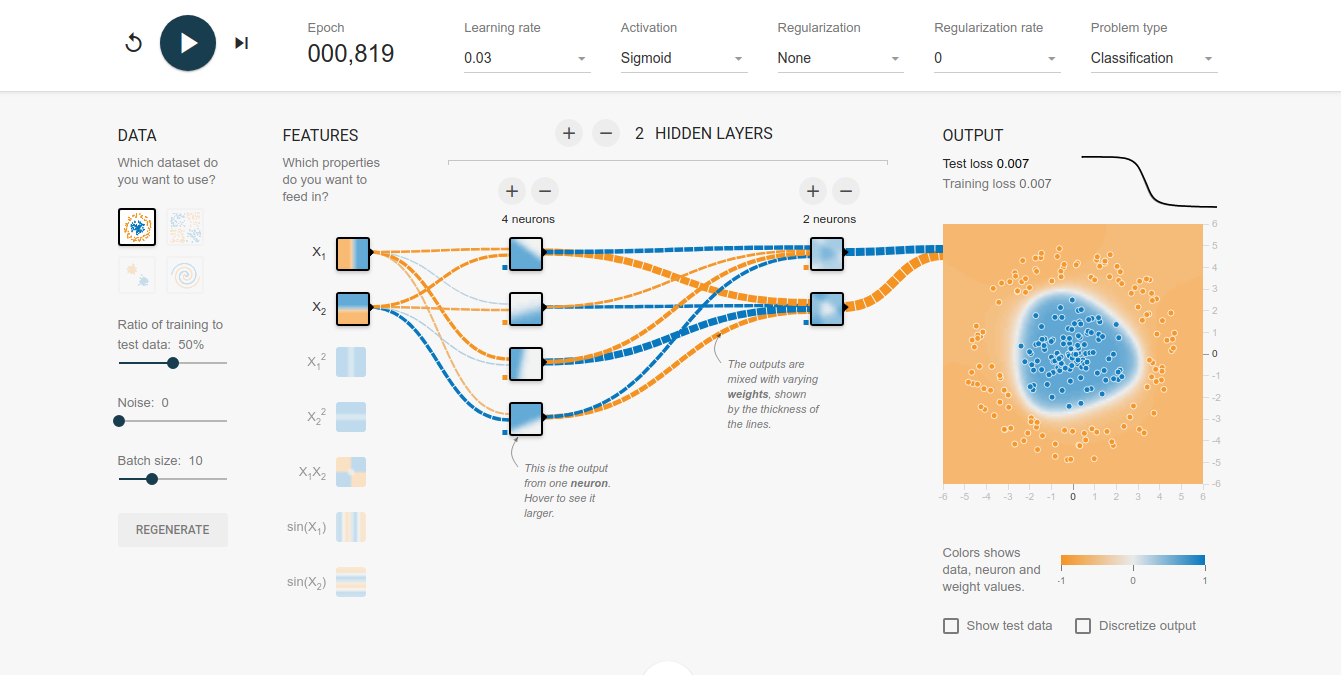
\includegraphics[width=\textwidth]{sigmoid.png}
                \caption{Training mit Sigmoid-Transferfunktion}
            \end{figure}
            \begin{figure}[H]
                \centering
                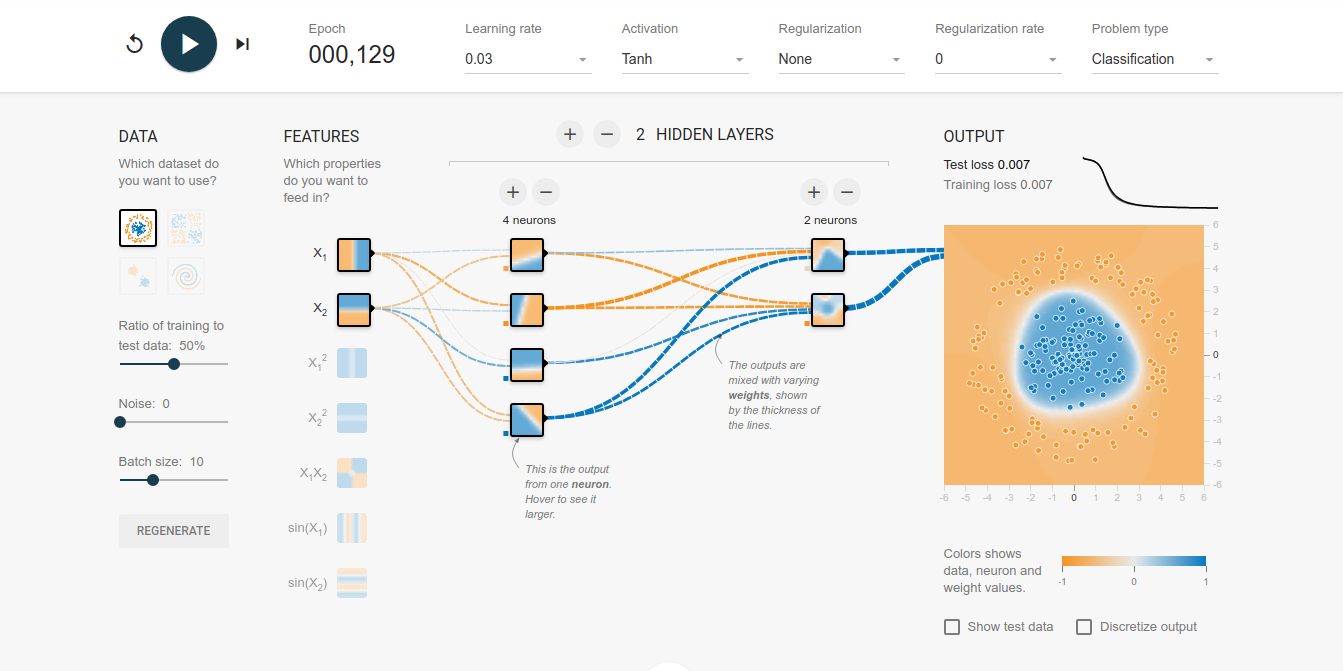
\includegraphics[width=\textwidth]{tanh.png}
                \caption{Training mit Tanh-Transferfunktion}
            \end{figure}
            \begin{figure}[H]
                \centering
                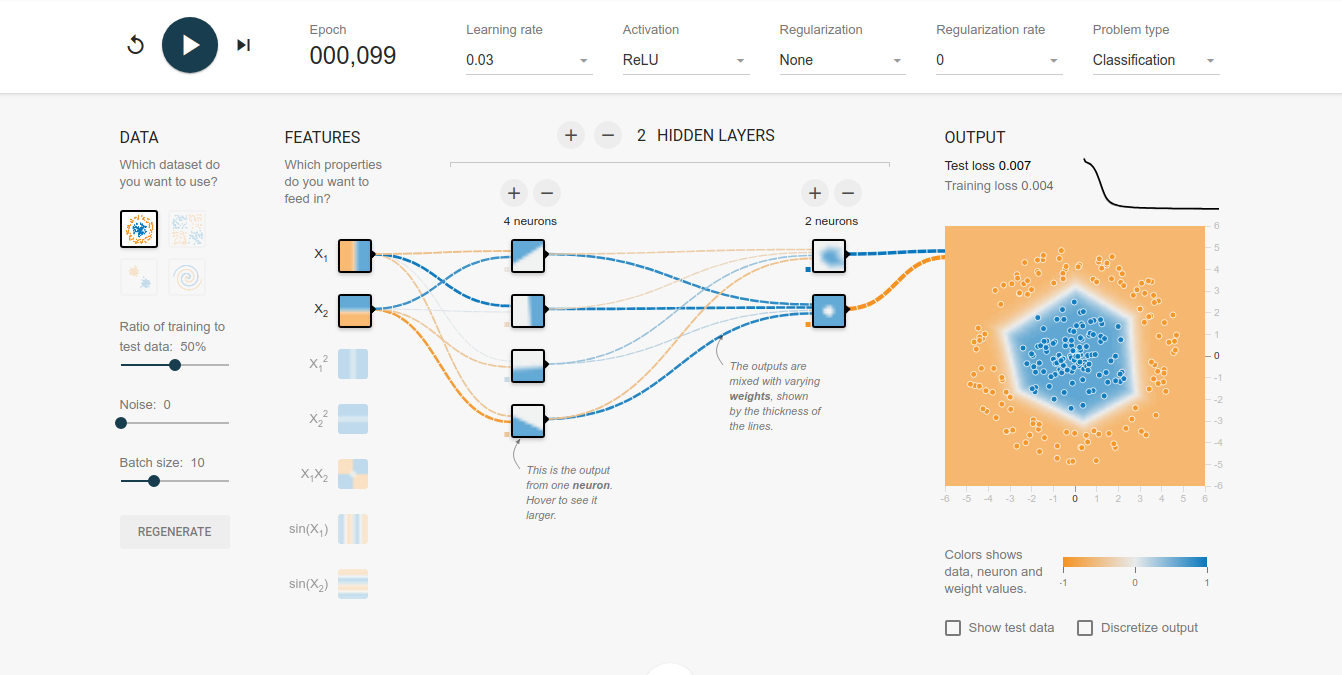
\includegraphics[width=\textwidth]{relu.png}
                \caption{Training mit ReLU-Transferfunktion}
            \end{figure}
        \item $ $
            \begin{figure}[H]
                \centering
                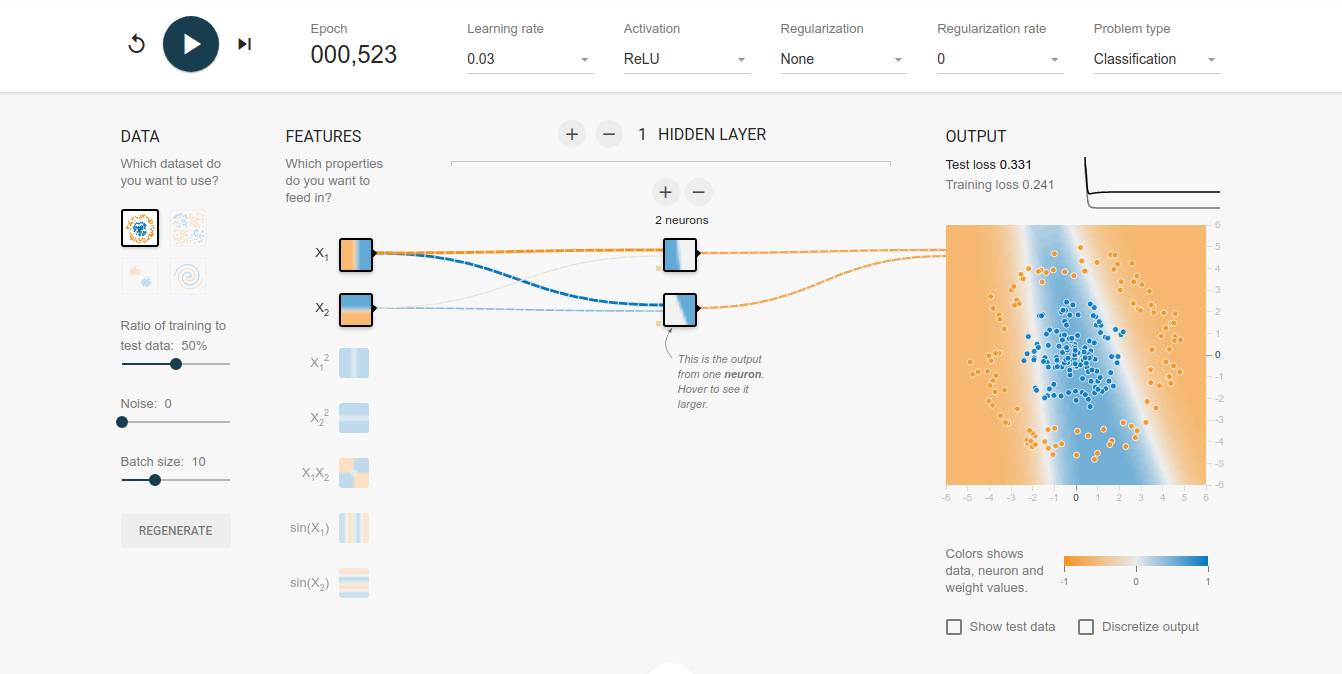
\includegraphics[width=\textwidth]{dying_relu.png}
                \caption{Dying Relu}
            \end{figure}
    \end{enumerate}

    \subsection{}
    \begin{enumerate}[label=\alph*)]
        \item $ $
            \begin{enumerate}[label=\roman*.]
                \item Die Varianz der Ausgangswerte jeden Layers nimmt bei fast allen Aktivierungsfunktionen ab. Die einzige Ausnahme stellt die SELU-Funktion dar.
                    Bei dieser Funktion geht die Varianz gegen 1.

                    Auch bei den Gradienten ist die Varianz im Falle der SELU-Aktivierung deutlich größer, bei allen anderen Aktivierungsfunktionen ist die Varianz des Gradienten sehr klein, bleibt aber über alle Layer hinweg relativ konstant. Bei der SELU-Funktion nimmt die Varianz der Gradienten über die Layer hinweg ab, ebenso der Mittelwert.
                \item Bei der Verteilung der Netzwerk-Aktivität ist der Mittelwert mit ReLU bzw. ELU Aktivierung in den ersten Layern positiv. Bei der Aktivierung mit $\tanh$ bzw. SELU ist der Mittelwert über alle Layer quasi $0$.

                    Bei der Verteilung des Gradienten lässt sich kein Unterschied erkennen. Die einzige Ausnahme bildet die Verteilung der Gradienten des Netzwerks mit SELU-Aktivierung hier wird der Mittelwert des Gradienten für weiter hinten gelegene Layer kleinie Verteilung der Gradienten des Netzwerks mit SELU-Aktivierung hier wird der Mittelwert des Gradienten für weiter hinten gelegene Layer kleiner.
                \item TODO
                \item In der ersten Epoche wird durch die SELU-Aktivierung am meisten gelernt. Der Betragsmäßige-Erwartungswert des Gradienten ist in allen Layer größer als bei den anderen Aktivierungsfunktionen, dadurch werden die Gewichte am stärksten adaptiert.allen Layer größer als bei den anderen Aktivierungsfunktionen, dadurch werden die Gewichte am stärksten adaptiert.
            \end{enumerate}
        \item 
            Das Histogramm der Aktivierungen mit $\tanh$ sind symmetrisch. Die Varianz nimmt für weiter hinten gelegene Schichten im Netz ab. Die ELU-Funktion verhält sich sehr ähnlich.

            Für die ReLU-Aktivierung ist zu sehen, dass kein Layer einen negativen Ausgangswert hat. Im Vergleich zur $\tanh$-Funktion ist die Varianz deutlich kleiner und nimmt über ab.

            Die Histogramme der Aktivierungen mit SELU-Funktionen sind deutlich breiter verteilt. Die Verteilung ist nicht symmetrisch, bleibt aber über alle Layer quasi konstant.
    \end{enumerate}
\end{document}
